% ---------------------------------------------------------------------------
% Author guideline and sample document for EG publication using LaTeX2e input
% D.Fellner, v1.20, Jan 18, 2023

\documentclass{egpubl}
\usepackage{eg2025}
\usepackage[T1]{fontenc}
\usepackage{graphicx}
\usepackage{dfadobe}  
\usepackage{tikz}
\usepackage{overpic}
\usepackage{amsmath}
\usepackage{amssymb}
\usepackage{float}
\usepackage{cite}  % comment out for biblatex with backend=biber
\usetikzlibrary{arrows, decorations.markings, arrows.meta,positioning,shadows,shapes.geometric,automata,positioning,fit,arrows.meta,calc,bending}
 
% --- for  Annual CONFERENCE
% \ConferenceSubmission   % uncomment for Conference submission
% \ConferencePaper        % uncomment for (final) Conference Paper
% \STAR                   % uncomment for STAR contribution
% \Tutorial               % uncomment for Tutorial contribution
% \ShortPresentation      % uncomment for (final) Short Conference Presentation
% \Areas                  % uncomment for Areas contribution
% \Education              % uncomment for Education contribution
\Poster                 % uncomment for Poster contribution
% \DC                     % uncomment for Doctoral Consortium
%
% --- for  CGF Journal
% \JournalSubmission    % uncomment for submission to Computer Graphics Forum
% \JournalPaper         % uncomment for final version of Journal Paper
%
% --- for  CGF Journal: special issue
% \SpecialIssueSubmission    % uncomment for submission to , special issue
% \SpecialIssuePaper         % uncomment for final version of Computer Graphics Forum, special issue
%                          % EuroVis, SGP, Rendering, PG
% --- for  EG Workshop Proceedings
% \WsSubmission      % uncomment for submission to EG Workshop
% \WsPaper           % uncomment for final version of EG Workshop contribution
% \WsSubmissionJoint % for joint events, for example ICAT-EGVE
% \WsPaperJoint      % for joint events, for example ICAT-EGVE
% \Expressive        % for SBIM, CAe, NPAR
% \DigitalHeritagePaper
% \PaperL2P          % for events EG only asks for License to Publish

% --- for EuroVis 
% for full papers use \SpecialIssuePaper
% \STAREurovis   % for EuroVis additional material 
% \EuroVisPoster % for EuroVis additional material 
% \EuroVisShort  % for EuroVis additional material
% \MedicalPrize  % uncomment for Medical Prize (Dirk Bartz) contribution, since 2021 part of EuroVis

% Licences: for CGF Journal (EG conf. full papers and STARs, EuroVis conf. full papers and STARs, SR, SGP, PG)
% please choose the correct license
%\CGFStandardLicense
%\CGFccby
%\CGFccbync
%\CGFccbyncnd

% !! *please* don't change anything above
% !! unless you REALLY know what you are doing
% ------------------------------------------------------------------------
\usepackage[T1]{fontenc}
\usepackage{dfadobe}  

\usepackage{cite}  % comment out for biblatex with backend=biber
% ---------------------------
%\biberVersion
\BibtexOrBiblatex
%\usepackage[backend=biber,bibstyle=EG,citestyle=alphabetic,backref=true]{biblatex} 
%\addbibresource{egbibsample.bib}
% ---------------------------  
\electronicVersion
\PrintedOrElectronic
% for including postscript figures
% mind: package option 'draft' will replace PS figure by a filename within a frame
% \ifpdf \usepackage[pdftex]{graphicx} \pdfcompresslevel=9
% \else \usepackage[dvips]{graphicx} \fi

\usepackage{egweblnk} 
% end of prologue

\title[EG poster]%
      {Markerless Multi-person Pose Estimation and Motion Synthesis for Combat Sports}

% for anonymous conference submission please enter your SUBMISSION ID
% instead of the author's name (and leave the affiliation blank) !!
% for final version: please provide your *own* ORCID in the brackets following \orcid; see https://orcid.org/ for more details.
\author[Hossein]
{\parbox{\textwidth}{\centering 
        Hossein Feiz$^1$, David Labbé$^1$, Sheldon Andrews$^1$
        }
        \\
{\parbox{\textwidth}{\centering 
        $^1$École de technologie supérieure (ETS), Montreal, Canada
       }
}
}
% ------------------------------------------------------------------------

% if the Editors-in-Chief have given you the data, you may uncomment
% the following five lines and insert it here
%
% \volume{36}   % the volume in which the issue will be published;
% \issue{1}     % the issue number of the publication
% \pStartPage{1}      % set starting page


%-------------------------------------------------------------------------
\begin{document}

% uncomment for using teaser
% \teaser{
%  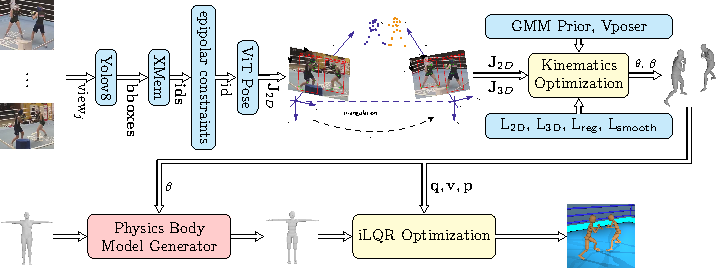
\includegraphics[width=0.9\linewidth]{pipeline.pdf}
%  \centering
%   \caption{The pipeline begins with generating bounding boxes  and robust tracking  for each individual in the scene. These tracking results are used to produce 2D poses. The triangulation process, produces smooth 3D keypoints. The kinematics optimization step incorporates the 2D and 3D keypoints, to create the SMPL parameters ($\mathbf{\theta}$, $\mathbf{\beta}$). The 3D relative joint positions, initial pose state  and velocity state of the humanoid, serve as a reference for a dynamic optimizer to correct any artifacts in the motion.}
% \label{fig:teaser}
% }

\maketitle
%-------------------------------------------------------------------------

\begin{abstract}
   Combat sports pose significant challenges for motion capture due to dynamic interactions and crowded backgrounds. Traditional methods like optical marker tracking, IMU-based solutions are not practical due to their intrusive nature, and Monocular vision-based approaches are affected by occlusions, encouraging the development of a multi-stage, multi-view tracking pipeline. This pipeline utilizes kinematic optimization to fuse 2D keypoints from multiple cameras, followed by physics-based trajectory optimization using model predictive control to enhance realism.
   Furthermore, leveraging interaction datasets attain from multi-view setup, the pipeline supports multi-person motion synthesis. It employs a seq2seq model to generate interactions from sparse VR headset inputs, and a diffusion prior model to generate the whole body poses. Finally, latent optimization ensures motions adhere to motion prior and satisfies high level criteria by producing controllable animations, suitable for combat sports analysis and training applications.

\begin{CCSXML}
<ccs2012>
<concept>
<concept_id>10010147.10010371.10010352.10010381</concept_id>
<concept_desc>Computing methodologies~Pose Estimation</concept_desc>
<concept_significance>300</concept_significance>
</concept>
<concept>
<concept_id>10010147.10010371.10010352.10010382</concept_id>
<concept_desc>Computing methodologies~Motion synthesis</concept_desc>
<concept_significance>300</concept_significance>
</concept>
</ccs2012>
\end{CCSXML}

\ccsdesc[300]{Computing methodologies~Pose Estimation}
\ccsdesc[300]{Computing methodologies~Motion synthesis}


\printccsdesc   
\end{abstract}  
%-------------------------------------------------------------------------
\section{Introduction}
We propose a multi-stage, multi-view tracking pipeline that uses kinematic and dynamics optimization to fuse 2D keypoints from multiple cameras. Additionally, our pipeline supports multi-person motion synthesis using interaction datasets from a multi-view tracking pipeline, employing a seq2seq model to generate interactions from sparse VR headset inputs and a diffusion prior model to produce whole-body poses. Latent optimization ensures that the motions adhere to motion priors and meet high-level criteria, making the system suitable for combat sports analysis and training.
\section{Pose Estimation}

\textbf{Tracking 2D and 3D Data:} Using epipolar constraints and long-term video object segmentation we produce consistent ids for everyone, these ids are used to produce 2D joints positions for tracking targets, we then use linear triangulation and Kalman estimation to produce robust 3D joints positions for each individual even in the presence of noise and outliers.   

\textbf{Kinematics Optimization:} The kinematics optimization focuses on refining the pose estimation of athletes using 2D and 3D keypoint data. Employing the SMPL model, the optimization aims to minimize the disparity between model joints and observed data while ensuring temporal coherence and natural movement. This is achieved through a comprehensive objective function that includes terms for smoothness, similarity to human motion priors, and alignment with both 2D re-projection evidence and triangulated 3D keypoints.

Initially, the optimization initializes shape parameters ($\beta \in \mathbb{R}^{10}$) of the SMPL model based on 3D keypoints obtained through triangulation. Subsequently, it iteratively adjusts shape and pose parameters ($\theta \in \mathbb{R}^{72}$) to refine the pose estimation.

Key components of the objective function include:
\begin{figure*}[htp]
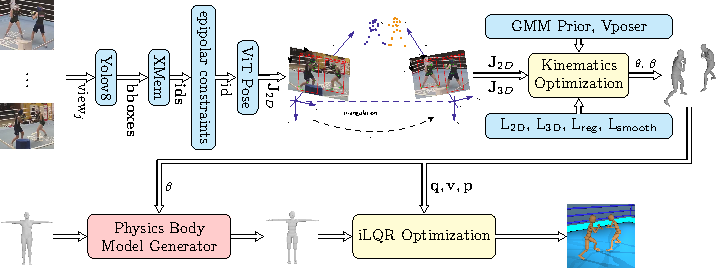
\includegraphics[width=0.73\linewidth]{pipeline.pdf}
 \centering
  \caption{The pipeline begins with generating bounding boxes  and robust tracking  for each individual in the scene. These tracking results are used to produce 2D poses. The triangulation process, produces smooth 3D keypoints. The kinematics optimization step incorporates the 2D and 3D keypoints, to create the SMPL parameters ($\mathbf{\theta}$, $\mathbf{\beta}$). The 3D relative joint positions, initial pose state  and velocity state of the humanoid, serve as a reference for a dynamic optimizer to correct any artifacts in the motion.}
\end{figure*}
\begin{itemize}
    \item \textbf{2D Re-projection Loss} ($\mathrm{L}_\text{2D}$): Aligns 3D joints with 2D joints across multiple camera views, emphasizing joints with high-confidence detections using a robust error function.
    \item \textbf{3D Alignment Loss} ($\mathrm{L}_\text{3D}$): Computes the Euclidean distance between predicted 3D joint positions and triangulated 3D keypoints, weighted by their confidence scores.
    \item \textbf{Smoothness Loss} ($\mathrm{L}_\text{smooth}$): Promotes consistency in pose transitions over time frames and vertices of the posed mesh.
    \item \textbf{Prior Losses} ($\mathrm{L}_{\text{GMM}}$, $\mathrm{L}_{\text{Vposer}}$): Introduces Gaussian Mixture Model (GMM) and Vposer priors to penalize unnatural poses, guiding the optimization towards more realistic and fluid motion.
\end{itemize}
 This comprehensive approach ensures accurate and lifelike pose estimation suitable for applications in sports biomechanics and animation.

%-------------------------------------------------------------------------

\textbf{Dynamics Optimization:} Output motion of the kinematics optimization contains high-frequency artifacts. To mitigate this, a second stage employs dynamics optimization using a physics-based humanoid model. This model, derived from joint positions and landmarks of an SMPL mesh, creates an articulated rigid-body structure with capsule collision geometry, featuring 56 joint-angle degrees of freedom and a 6 degree of freedom root joint.

The dynamics optimization stage aims to refine motion trajectories by considering joint torques and biomechanical constraints within a physical environment. It computes joint torques using an iterative Linear Quadratic Regulator (iLQR) algorithm, which optimizes control inputs to smooth and stabilize motion trajectories. This approach accounts for contact forces and body dynamics, enhancing the overall quality and naturalness of the generated motions by iteratively refining control trajectories over short time horizons.

\begin{figure}[htbp]
  \centering
  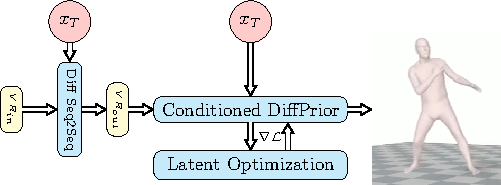
\includegraphics{condiffusion}
  \caption{motion synthesis pipeline}
    \label{fig:condtion-diffusion}
\end{figure}

Figure~\ref{fig:condtion-diffusion} illustrate the main components of the motion synthesis pipeline. The condition for the seq2seq model contains the VR sensor information of the player and the output is the corresponding synthetic VR information for the opponent at each sequence. The diffusion prior is conditioned on the opponent synthetic information and produces the whole body pose for the opponent. The optimization in loop makes sure the output motion has the desired trajectories based on a high-level loss function.



\section{Motion Synthesis}
%---------------------------------------------------------------------
\textbf{Diff Seq2Seq: Interaction Diffusion Model}
 
A novel application of sequence-to-sequence (seq2seq) models in virtual reality involves generating responsive opponent motions based on sparse VR input data. In this context, the seq2seq model trained on the interaction dataset translating the sparse signals captured from VR sensors into synthetic VR signals for the virtual opponents. Trained on a specialized multi-person boxing dataset, the model learns to map the sparse input, into coherent sequences of actions that simulate human-like behavior during a boxing match. By leveraging the dataset’s diverse scenarios and real-world motion variations, the seq2seq model not only predicts the opponent’s reactions but also adapts to different player actions, enhancing the realism and engagement of VR gaming experiences. This approach marks a significant advancement in interactive VR applications by bridging the gap between sparse sensor data and immersive virtual interactions.

%---------------------------------------------------------------------
\textbf{Conditioned Diffprior: Sparse inputs to whole body pose}
This approach overcomes the inherent challenges of accurately predicting smooth and realistic full-body motions with minimal input data. By leveraging a lightweight MLP architecture and employing a block-wise injection scheme for embedding time step information, the conditional diffusion model effectively reduces artifacts like jittering and enhances robustness against signal loss.
% The conditional diffusion model architecture optimizes computational efficiency while maintaining high accuracy in estimating full-body poses, making it suitable for immersive VR experiences demanding fluid and responsive interactions.

%---------------------------------------------------------------------
\textbf{Latent Optimization: Controlled motion synthesis}

Optimize noisy motion inputs directly in the latent space of the diffusion model. By treating motion denoising as a black box and iteratively adjusts the diffusion noise vector using gradients computed through an ODE solver, ensuring the output motion meets user-defined criteria. This approach avoids the need for fine-tuning models for specific tasks, demonstrating superior performance in motion editing, preservation, and task fulfillment compared to existing methods.

\end{document}
{}
